% -*- coding: utf-8; -*-

\chapter{Validação do problema}
\label{cha:Valida\c{c}\~{a}o do problema}

A validação do problema foi efetuada por meio de entrevistas com alunos de graduação do departamento de informática. As entrevistas tinham como objetivo obter as opiniões de diferentes alunos em diferentes períodos de suas graduações quanto as suas preferências ao realizar as suas matrículas. As opiniões são essenciais para planejar um algoritmo de recomendação que abrange as preferênciasdo máximo de estudantes.

\section{Método das entrevistas}

Os entrevistados são alunos de graduação dos cursos do departamento de informática da PUC-Rio, cursando os cursos de engenharia da computação ou de ciência da computação. Foram selecionados vários alunos em diferentes estágios da graduação, do segundo ao sexto ano de graduação. Como algumas perguntas se referem às escolhas de disciplinas eletivas, e essas só começam a ser escolhidas no meio do período de graduação, não foram escolhidos estudantes no primeiro ano de graduação. 

\section{Perguntas realizadas}
A seguir estão as seis perguntas realizadas para cada entrevistado do departamento de informática, assim como uma explicação do motivo da pergunta ser realizada.

% REMOVER A EXPLICAÇÃO DA LISTA
% E COLOCAR OS EXEMPLOS NA 5.3


\begin{enumerate}
    \item \textbf{Qual é o seu curso e período atual?} O período atual do entrevistado é utilizado para entender o contexto de suas respostas, pois é necessário observar se o período em que o graduando está altera sua opinião ao realizar a sua matrícula. Como a quantidade de períodos propostos para a conclusão do curso variam de curso para curso no departamento de informática, também foi solicitado ao entrevistado seu curso para entender seu progresso de estudo na universidade e entender ainda melhor o contexto das suas próximas respostas.
        
        %% \textit{"Eu sou aluno de engenharia de computação, atualmente no sétimo período."}
    
    \item \textbf{Em média quantos créditos você faz num semestre?} A quantidade de créditos por semestre é relevante para que o algoritmo de recomendação tenha um conhecimento da média de disciplinas selecionadas por período. Essa média pode ser usada pelo algoritmo para saber quantas disciplinas o estudante ainda pretende fazer naquele semestre e recomendar de acordo.
        %% \textit{"Nos últimos semestres eu tenho feito o limite máximo de 30 créditos, mas antes eu fazia uma média de 22 ou 24 créditos."}
    
    \item \textbf{Você se prepara com anteced\^encia para sua matr\'icula? Se sim, com quanta anteced\^encia? Se não, por quê?} Essa pergunta é fundamental para planejar uma expectativa de utilização da ferramenta de recomendação de disciplinas, pois a ferramenta com o algoritmo estaria disponibilizada em um sistema cujo obtivo é planejar a sua matr\'icula.
    
        %% \textit{"Sim, eu me prepararo assim que os horários das disciplinas são atualizados no microhorário. Normalmente dois dias antes da minha matrícula, eu já tenho algumas escolhas reservadas."}
    
    \item \textbf{Que crit\'erios você utiliza para escolher uma disciplina? Dados os critérios fornecidos, coloque-os em uma ordem de mais relevante para menos relevante.} Essa é a pergunta mais fundamental para o planejamento do algoritmo. Afinal, o objetivo do algoritmo de recomendação é recomendar disciplinas relevantes para um aluno. Por isso, é necessário saber o que torna uma disciplina relevante para ser escolhida.
        
        %% RESPOSTA INSERIDA NA PROXIMA SECÇÃO:
        %% \textit{"Eu acho que a matéria em si, se ela é mais difícil de entender ou mais fácil, e também o método de avaliação daquela disciplina, ou seja, se a nota final é composta de somente duas provas, ou se são vários pequenos trabalhos espalhados pelo semestre. Além disso, eu diria que o horário também é um limitador, porque não consigo ter aula sete da manhã todos os dias. Mas eu acho que o mais importante para mim é o professor: Se eu sei quem é o professor, sei que ele explica bem, vale a pena mesmo que a matéria seja mais difícil. Eu diria que a ordem dos critérios seria o professor, depois a matéria em si, depois o método de avaliação e por último o horário da disciplina."}

    \item \textbf{Como você procura disciplinas eletivas?} O objetivo dessa pergunta é descobrir como cada estudante procura as disciplinas eletivas, para saber quais são as principais fontes de informações utilizadas.
        
        %% \textit{"Eu normalmente procuro pela listagem completa das disciplinas do departamento, oferecida através do microhorário. Também havia uma lista de disciplinas eletivas oferecidas no próximo período que era enviada por email, mas esta nunca mais foi enviada ou atualizada."}

    \item \textbf{Você, pessoalmente, prefere disciplinas mais fáceis, mas que talvez não sejam muito úteis para a sua carreira, ou disciplinas mais relevantes mas que possam ser mais difíceis?} Essa pergunta pretende entender qual das duas opções é mais frequente. Caso a maioria dos estudantes preferem disciplinas mais fáceis, o algoritmo irá depender mais das notas dos alunos, e não tanto do conteúdo da disciplina em si. Caso a maioria dos estudantes preferem disciplinas mais relevantes, por exemplo.
    
        %% RESPOSTA INSERIDA NA PROXIMA SECÇÃO:
        %% \textit{"Eu prefiro [disciplinas] eletivas mais fáceis, porque eu as vejo como uma oportunidade para facilitar a minha vida na faculdade, pois já tenho outras disciplinas mais difíceis para me preocupar. Eu encaro as [disciplinas] eletivas como um escape para poder respirar."}

\end{enumerate}

Ao final da entrevista, também foi oferecida a oportunidade de fornecer alguma opinião sobre o sistema de recomendação a ser desenvolvido.

\section{Resultados das entrevistas}

\subsection{Dados básicos dos estudantes (Perguntas 1 e 2)}

Dos onze entrevistados, cinco eram alunos de ciência de computação e os outros seis eram de engenharia de computação. 5 dos 6 alunos entrevistados de engenharia de computação já haviam cursado mais da metade do curso (já cursou 5 dos 10 semestres recomendados), e 3 dos 5 alunos entrevistados de ciência de computação já haviam cursado mais da metade do curso (já cursou 4 dos 8 semestres recomendados). Além disso, dos onze alunos, nove eram homens e dois eram mulheres.

A distribuição dos períodos atuais dos entrevistados pode ser visualizada na figura \ref{fig:entrevista-grafico}. 

\begin{figure}[!ht]
    \begin{center}
    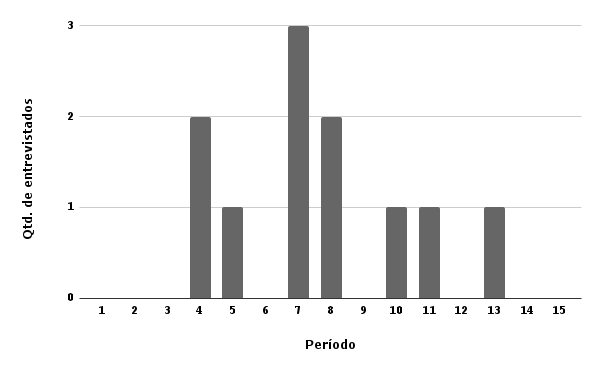
\includegraphics[width=350pt]{figuras/grafico-entrevista}
    \caption{Distribuição da quantidade de entrevistados pelos seus períodos atuais.}
    \label{fig:entrevista-grafico}
    \end{center}
  \end{figure}
  
A quantidade média de créditos por semestre dos alunos entrevistados é de 24 créditos, semelhante à quantidade média de créditos por semestre no currículo recomendado de ambos os cursos.

\subsection{Escolha de disciplinas (Perguntas 3 e 4)}
\label{sec:escolha-disciplinas}

Dez dos onze entrevistados se preparam com antecedência para a matrícula. Três desses utilizam como base o repositório de disciplinas microhorário para buscar as informações das disciplinas oferecidas para o pŕoximo período, e também utilizam o microhorário para descobrir quais são as disciplinas eletivas disponibilizadas no período. Todos os dez entrevistados utilizam o simulador de matrícula para confirmar suas escolhas. Apenas um dos entrevistados não se prepara com antecedência, fazendo suas pesquisas e escolhas durante o período da própria matrícula. 

Os critérios preferidos de cada aluno variam bastante. Por exemplo, um entrevisto citou que alguns critérios são  \textit{"a matéria em si, se ela é mais difícil de entender ou mais fácil, e também o método de avaliação, ou seja, se a nota final é composta de somente duas provas, ou se são vários trabalhos pequenos espalhados pelo semestre. Além disso, eu diria que o horário também é um limitador, porque não consigo ter aula sete da manhã todos os dias. Mas eu acho que o mais importante para mim é o professor: Se eu sei quem é o professor, sei que ele explica bem, vale a pena mesmo que a matéria seja mais difícil. Eu diria que a ordem dos critérios seria o professor, depois a matéria em si, depois o método de avaliação e por último o horário da disciplina."}.

Como pode ser observado na resposta fornecida acima, as respostas podem variar bastante de aluno para aluno. Por isso, os critérios de escolha de disciplinas ditos nas entrevistas foram agrupados em cinco grupos: (1) Conteúdo da disciplina; (2) Professor; (3) Método de avaliação; (4) Horário da disciplina e (5) Opinião de amigos. A tabela \ref{tab:entrevista-criterios-raw} com as respostas dos onze entrevistados e as suas respostas. O número indica em qual posição ficou aquele critério na ordem de preferência pessoal do aluno.

\begin{table}[!ht]
    \begin{center}
        \begin{tabular}{ l|c|c|c|c|c } 
            & Conteúdo & Professor & Avaliação & Horário & Opinião \\ 
            \hline 
            \textit{Entrevistado 1 } & 3 & - & - & 1 & 2 \\     % miguel angelus
            \textit{Entrevistado 2 } & 1 & - & - & 3 & 2 \\     % joao biscaia
            \textit{Entrevistado 3 } & 2 & 3 & - & - & 1 \\     % laura luz 
            \textit{Entrevistado 4 } & 3 & 1 & - & 2 & - \\     % thomas botelho
            \textit{Entrevistado 5 } & 2 & - & - & 1 & 3 \\     % rafael lavatori
            \textit{Entrevistado 6 } & 1 & - & - & - & - \\     % antenor bastos
            \textit{Entrevistado 7 } & 1 & - & - & - & - \\     % jeronimo soares
            \textit{Entrevistado 8 } & 2 & 3 & 1 & 4 & - \\     % mariana barreto
            \textit{Entrevistado 9 } & 3 & 2 & - & - & 1 \\     % paulo de tarso
            \textit{Entrevistado 10} & 1 & - & 3 & 2 & - \\     % luiz fellipe
            \textit{Entrevistado 11} & - & 2 & - & 1 & - \\     % miguel
        \end{tabular}
    \end{center}
    \caption{Graus dos critérios de escolhas de disciplinas escolhidos pelos 
    entrevistados}
    % O número indica o grau de importância, onde 1 é o mais importante. Os critérios sem números são critérios não citados pelo entrevistado na entrevista.
    
    \label{tab:entrevista-criterios-raw}
\end{table}

Para gerar uma comparação dos critérios, foi dado um peso para cada grau de importância de acordo com a tabela \ref{tab:grau-peso}.

\begin{table}[!ht]
    \begin{center}
        \begin{tabular}{ r||c|c|c|c|c|c } 
            \textit{Grau} & 1 & 2 & 3 & 4 & 5 & - \\
            \hline 
            \textit{Peso} & 5 & 4 & 3 & 2 & 1 & 0 \\
        \end{tabular}
    \end{center}
    \caption{Relação de peso para grau dos critérios de escolhas}
    \label{tab:grau-peso}
\end{table}

Ao substituir os pesos da Tabela \ref{tab:grau-peso} na Tabela \ref{tab:entrevista-criterios-raw}, é possível somar os pesos para cada critério de escolha e obter uma relação entre eles, conforme a tabela \ref{tab:entrevista-criterios-peso}.

\begin{table}[!ht]
    \begin{center}
        \begin{tabular}{ l|c|c|c|c|c } 
            & Conteúdo & Professor & Avaliação & Horário & Opinião \\ 
            \hline 
            \textit{Entrevistado 1 } & 3 & 0 & 0 & 5 & 4 \\     % miguel angelus
            \textit{Entrevistado 2 } & 5 & 0 & 0 & 3 & 4 \\     % joao biscaia
            \textit{Entrevistado 3 } & 4 & 3 & 0 & 0 & 5 \\     % laura luz 
            \textit{Entrevistado 4 } & 3 & 5 & 0 & 4 & 0 \\     % thomas botelho
            \textit{Entrevistado 5 } & 4 & 0 & 0 & 5 & 3 \\     % rafael lavatori
            \textit{Entrevistado 6 } & 5 & 0 & 0 & 0 & 0 \\     % antenor bastos
            \textit{Entrevistado 7 } & 5 & 0 & 0 & 0 & 0 \\     % jeronimo soares
            \textit{Entrevistado 8 } & 4 & 3 & 5 & 2 & 0 \\     % mariana barreto
            \textit{Entrevistado 9 } & 3 & 4 & 0 & 0 & 5 \\     % paulo de tarso
            \textit{Entrevistado 10} & 5 & 0 & 3 & 4 & 0 \\     % luiz fellipe
            \textit{Entrevistado 11} & 0 & 4 & 0 & 5 & 0 \\     % miguel
            \hline
            \textbf{Soma}            & 41& 19& 8 & 28& 21 
        \end{tabular}
    \end{center}
    \caption{Pesos dos critérios de escolhas de disciplinas escolhidos pelos entrevistados.}
    %  O número indica o valor relativo ao grau de importância, onde 5 é o mais importante.
    \label{tab:entrevista-criterios-peso}
\end{table}

Observando a Tabela \ref{tab:entrevista-criterios-peso}, as somas dos pesos indicam que a ordem dos critérios mais relevantes na escolha de uma disciplina, do mais relevante para o menos relevante:
\textit{Conteúdo da disciplina}, \textit{Horário da disciplina}, \textit{Opinião de amigos}, \textit{Professor} e \textit{Método de avaliação}.

\subsection{Disciplinas eletivas (Perguntas 5 e 6)}

Dos onze entrevistados, nove citaram a utilização do microhorário para coletar as disciplinas eletivas do período. Os outros dois dependem mais de recomendação de amigos. Três entrevistados procuram por uma listagem oficial de disciplinas eletivas oferecidas pelo departamento para o próximo período, mas nem sempre encontram essa listagem oficial.

Por último, quatro entrevistados preferem disciplinas eletivas mais fáceis, enquanto três entrevistados preferem disciplinas eletivas que sejam mais relevantes para a sua formação. Os quatro restantes preferem um equilíbrio de facilidade e relevância. Dois entrevistados disseram que inicialmente escolhem disciplinas mais relevantes, mas que ao decorrer dos períodos optam por eletivas mais fáceis. Uma das respostas foi que \textit{"[Eu] prefiro [disciplinas] eletivas mais fáceis, porque eu as vejo como uma oportunidade para facilitar a minha vida na faculdade, pois já tenho outras disciplinas mais difíceis para me preocupar. Eu encaro as [disciplinas] eletivas como um escape para poder respirar."}
